% No Free Null: Reference Distributions for Explaining
% Reinforcement Learning Agents
% Workshop version, cut from main.tex.
%
% Four pages of body, with the bibliography running onto a fifth. That is the
% shape most workshops ask for ("4 pages excluding references"); a venue that
% counts references needs roughly one more column cut, and the ground-truth
% subsection is the one to lose.
%
% Dropped relative to the full version: the power curve, the certified-ranking
% result, integrated gradients, credit-assignment robustness, the horizon
% experiment, the off-manifold analysis, the null-construction audit, and the
% cold-rebuild reproduction. Those are the extensions; what remains is the
% argument.
%
% Build:  tectonic workshop.tex

\documentclass[10pt,twocolumn]{article}

\usepackage[letterpaper,margin=0.75in,columnsep=0.28in]{geometry}
\usepackage[T1]{fontenc}
\usepackage[utf8]{inputenc}
\usepackage{amsmath,amssymb}
\usepackage{graphicx}
\usepackage{booktabs}
\usepackage{microtype}
\usepackage{caption}
\usepackage[hidelinks]{hyperref}
\usepackage[numbers,sort&compress]{natbib}
\usepackage{titlesec}
\usepackage{enumitem}

\captionsetup{font=small,labelfont=bf,skip=4pt}
\titlespacing*{\section}{0pt}{7pt}{3pt}
\titlespacing*{\subsection}{0pt}{5pt}{2pt}

% headings set ragged-right rather than justified. at column width a justified
% heading hyphenates ("does not trans-fer"), which reads as a typo.
\titleformat*{\section}{\large\bfseries\raggedright}
\titleformat*{\subsection}{\normalsize\bfseries\raggedright}
\setlength{\parskip}{0pt}
\setlength{\abovedisplayskip}{4pt}
\setlength{\belowdisplayskip}{4pt}
% every table here is 4 numeric columns in a 3.35in column. at the 6pt default
% all three overrun the text block by a few points.
\setlength{\tabcolsep}{3.5pt}

\newcommand{\vfn}{v}

\title{\vspace{-1.6em}\bfseries No Free Null: Reference Distributions for Explaining\\Reinforcement Learning Agents}
% Replace with the venue's anonymous block if submitting double-blind.
\author{Aaryan Singh\\[2pt]
  \normalsize Independent Researcher\\[1pt]
  \normalsize\texttt{singha9@rose-hulman.edu}}
\date{}

\begin{document}

\twocolumn[
  \begin{@twocolumnfalse}
  \maketitle
  \vspace{-2.0em}  % \maketitle reserves space for a date line that is empty
  \begin{quote}
  \small
  \textbf{Abstract.}
  Deciding whether an explanation of a reinforcement learning agent means
  anything requires a reference distribution: what it would have looked like had
  the agent learned nothing. Reinforcement learning has no agreed way to build
  one, and the problem is harder than it appears. The construction the field
  already uses, randomising network parameters, has almost no power: across
  sixteen checkpoints on four control tasks it never exceeds $z=2.45$, and its
  width \emph{equals} the standard deviation of random-initialisation return to
  three significant figures, so it measures the variance of initialisation
  rather than the explanation. We then build the three natural replacements and
  each fails differently. A signal-free corpus varies the corpus as well as the
  information. Blinding the observation channel removes the agent's capacity to
  respond, collapsing the reference onto a point mass and firing on a corpus
  built to contain no signal. Permuting the outcomes, the direct analogue of the
  supervised label-permutation test, leaves the price forecasting a label it no
  longer matches and hands the null agents an arbitrage worth \$49 an episode.
  Removing the information always perturbs something else, and the perturbation
  decides the verdict. We motivate this with an agent whose explanation is
  stable across seeds, semantically legible, and empty, and which can be driven
  from $39.9\%$ to $3.2\%$ of attribution mass at no measurable cost in return.
  \end{quote}
  \vspace{1.1em}
  \end{@twocolumnfalse}
]

\section{Introduction}

Interpretability is proposed as a basis for oversight: if we can see which
inputs drive a policy, we can decide whether to trust it. That needs an
attribution to mean something, and attribution methods return an answer whether
or not it does. Given any policy and state, Shapley
values~\citep{shapley1953value,lundberg2017unified} and integrated
gradients~\citep{sundararajan2017axiomatic} produce a ranked, signed vector.
Nothing in the output separates an attribution reflecting structure the agent
exploits from one reflecting nothing.

Telling them apart needs a \emph{reference distribution}: what the explanation
would have looked like had the agent learned nothing. Supervised learning has
two standard ones, both from \citet{adebayo2018sanity}: randomise the
parameters, or train on permuted labels. Reinforcement learning has adopted the
first and not the second. \citet{huber2022benchmarking} apply the parameter test
to Atari saliency and observe that the data-randomisation test has no obvious RL
analogue. The obstacle is structural rather than clerical: supervised labels can
be permuted while the input distribution is held exactly fixed, whereas an RL
agent's observations, actions and trajectories are all generated by the policy,
so there is no label to permute that leaves the rest of the problem untouched.

We set out to supply one. The result is negative and the negative result is the
contribution: parameter randomisation, repurposed to generate reference draws,
has almost no power, and each of the three natural replacements fails in its own
way. Kept in its original form as a similarity check the parameter test remains
sound, but it answers a different question, and on our two agents its verdicts
are the reverse of ours.

\paragraph{Contributions.}
\begin{enumerate}[leftmargin=1.2em,itemsep=1pt,topsep=2pt]
\item Parameter randomisation is a near-powerless reference in RL, and a variance
decomposition explains it: the span inherits the spread of random-initialisation
return, which it matches to three significant figures.
\item Three replacements, three distinct failures, each with a measured
mechanism.
\item A worked case of an explanation that passes every conventional check and
carries no information.
\item Attribution is not identified by task performance: it can be forged at a price
equal to the importance of the feature being hidden.
\end{enumerate}

\paragraph{What we do not claim.}
The argument that RL attribution should target outcomes rather than policy
outputs is due to \citet{beechey2023sverl}; FastSVERL~\citep{beechey2025fastsverl}
addresses the scalability, off-policy and temporal problems we only name. Our
test adapts \citet{adebayo2018sanity}. Deletion-based fidelity is established
practice in XRL~\citep{cheng2025survey,milani2024xrl}. Our contribution is the RL
construction, the demonstration that four of them fail and why, and the
consequences.

\section{Method}

Let $\vfn(S)$ be the expected episode return of an agent observing only the
features in $S \subseteq N$, with features outside $S$ replaced at every timestep
by draws from a reference distribution. Define the \emph{attribution span}
$\Delta = \vfn(N) - \vfn(\emptyset)$.

Shapley values and integrated gradients satisfy additivity identities under which
per-feature attributions sum to $\Delta$, so the span can be read off either. It
is worth stating that $\Delta$ is \emph{not} a Shapley quantity: it is the
difference between two masked rollouts and depends only on the masking. This has
a practical consequence: it costs two evaluations rather than $2^{|N|}$.

\begin{figure*}[t]
\centering
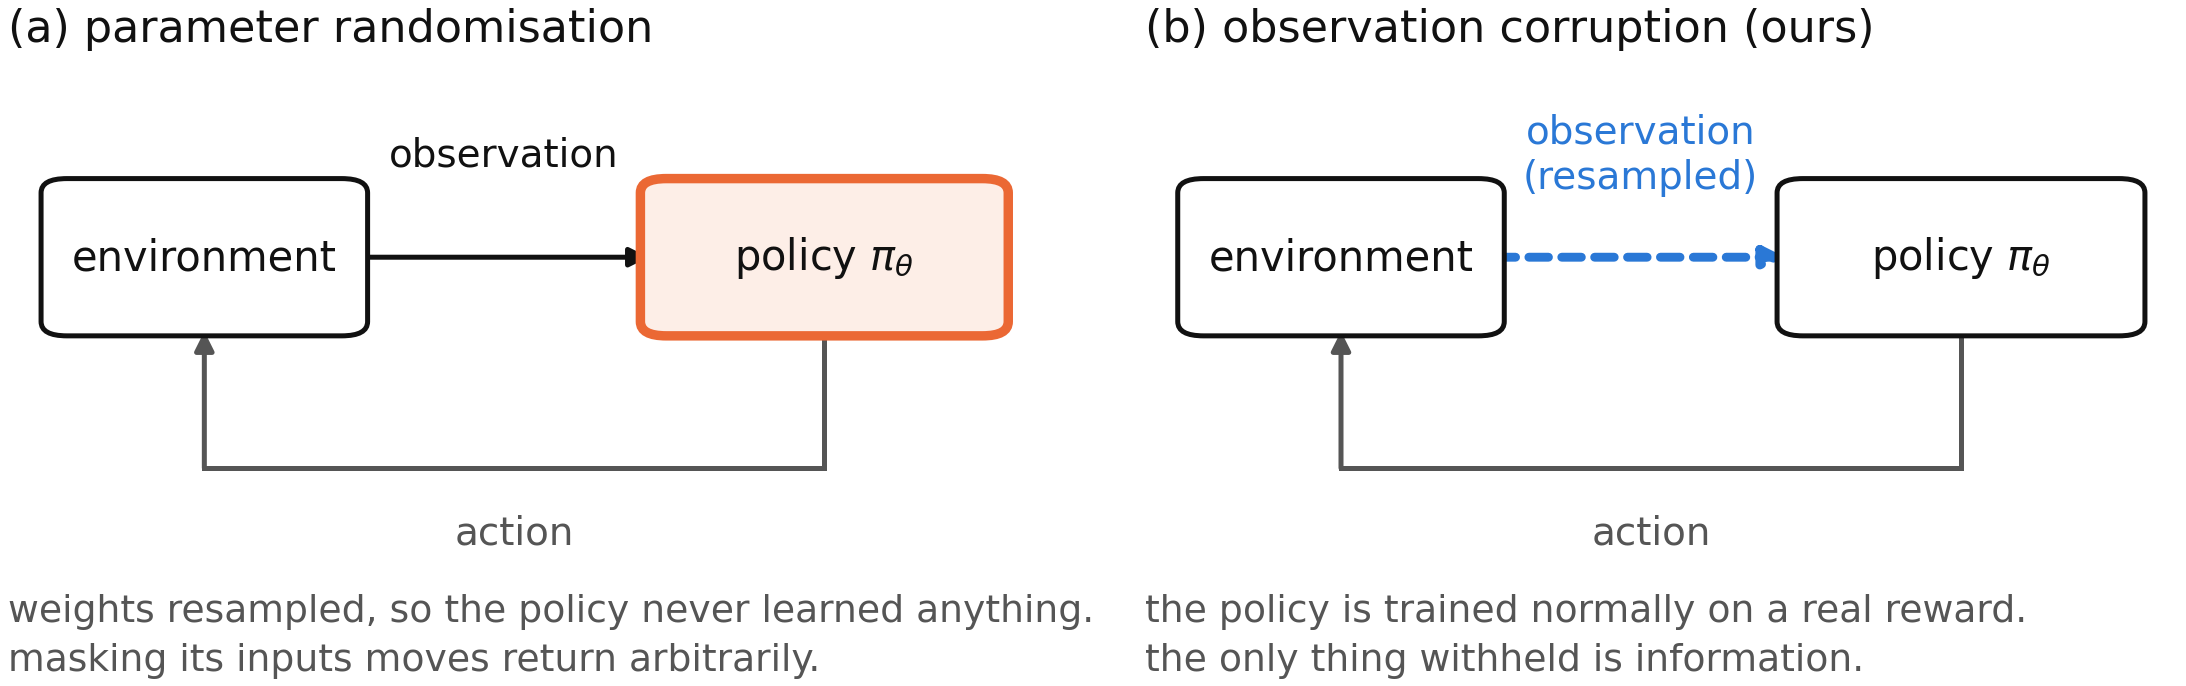
\includegraphics[width=\textwidth]{figures/fig_method.png}
\caption{Two ways to build a reference distribution of explanations for an agent
that learned nothing. The established check (a) randomises the policy's
parameters, leaving a network that was never trained. Ours (b) corrupts the
environment's observation channel instead, so the agent optimises a real reward
with nothing to condition on. Only (b) yields a normally trained policy, which
is the failure mode that occurs in deployment.}
\label{fig:method}
\end{figure*}

\medskip
\noindent\textbf{Blind-observation null.} \emph{Replace every observation with an
independent draw from a fixed distribution matched to the environment's
observation moments. Leave dynamics and reward untouched. Train normally}
(Figure~\ref{fig:method}).
\medskip

Such an agent faces the real task and receives real return but cannot condition
on anything. Unlike parameter randomisation it yields a \emph{normally trained}
policy: the failure mode that occurs in deployment. Matching the reference
moments matters, or the network fails for reasons of scale rather than
information.

Given null draws with mean $\bar\Delta$ and standard deviation $s$ we report a
rank $p$-value and $z = (\Delta_{\mathrm{obs}} - \bar\Delta)/s$, and require both
to reject. The rank statistic assumes no shape but bottoms out at $1/(n+1)$; the
normal statistic has resolution but assumes a shape the null need not have. If
every null draw is identical, $s=0$; we return $z=\pm\infty$ and surface the
degeneracy rather than guarding it away, but treat it as a reason to distrust
the reference. A point-mass null has no specificity, and building one is how a
more principled-looking null construction turned out to fire on a corpus with no
signal in it (Section~\ref{sec:cost}).

\section{Setup}

\paragraph{Environments with known answers.} Explanation evaluation lacks ground
truth~\citep{cheng2025survey}. We construct fixed-length synthetic corpora where
the answer is fixed by construction: a \emph{planted signal} (one of 18 features
informative about the outcome), a \emph{null} (none), and a \emph{decoy} (one
feature correlating $0.989$ with the outcome in-sample and $0.006$ out of
sample).

\paragraph{Market.} Our main setting is a binary contract settling to \$1.00 if
BTC is higher after 15 minutes, on a regulated prediction market: 6{,}425 settled
contracts over 68 days, walk-forward split by time, test evaluated once. Every
episode resolves to a known value. Agents are trained with
PPO~\citep{schulman2017ppo}; reward is the change in mark-to-market equity net of
the exchange's published fee schedule, a $9\%$ round-trip hurdle at the price
this contract trades at.

\paragraph{Control tasks.} CartPole-v1, Acrobot-v1, MountainCar-v0 and
Pendulum-v1, whose observation spaces are small enough to enumerate all
coalitions, so Shapley values there are exact. Pendulum's continuous action is
discretised into nine values so the same categorical PPO trains on every task.

\section{Results}

\subsection{An explanation that passes every check}

The market is empirically efficient: its implied probability has a weighted mean
absolute calibration error of $0.0172$, and spot return correlates $0.476$ with
the outcome but only $0.016$ with the residual after the price is accounted for.
No policy beats abstention (Table~\ref{tab:base}).

\begin{table}[t]
\centering\small
\caption{Test split, 1{,}284 held-out episodes. Paired bootstrap against
always-flat.}
\label{tab:base}
\begin{tabular}{lrrr}
\toprule
Policy & Mean P\&L & Trades/ep & $p$ vs flat \\
\midrule
always-flat & $+0.000$ & 0.00 & n/a \\
buy-and-hold & $-1.608$ & 1.00 & 0.23 \\
\textbf{PPO} (5 seeds) & $\mathbf{-0.595 \pm 0.176}$ & 1.37 & \textbf{0.10} \\
mean-reversion & $-11.615$ & 4.94 & $<$0.0001 \\
random & $-18.532$ & 9.33 & $<$0.0001 \\
\bottomrule
\end{tabular}
\end{table}

PPO's shortfall is its own: on synthetic data with no signal by construction the
same agent scores $-0.47 \pm 0.47$. Yet across five seeds whose pairwise
performance differences are indistinguishable in all ten pairs, its attributions
have cross-seed rank correlation $0.849$ with $100\%$ agreement on the top
feature, a top-5 ranking whose adjacent gaps exceed their combined standard
errors, and a legible story: time-to-expiry dominates, reading as an agent that
learned when not to trade.

The null test disagrees (Table~\ref{tab:null}, Figure~\ref{fig:null}). It has
power and specificity, and the market agent sits at the centre of the
distribution of explanations of nothing.

\begin{table}[t]
\centering\small
\caption{Null-model test. Null from 24 blind-trained agents, span
$+8.19 \pm 5.11$.}
\label{tab:null}
\begin{tabular}{lrrl}
\toprule
Case & Span & $z$ & Verdict \\
\midrule
planted signal & $+70.89$ & $\mathbf{+12.27}$ & informative \\
null corpus & $+11.86$ & $+0.72$ & not distinguishable \\
\textbf{real market} & $\mathbf{+9.37}$ & $\mathbf{+0.23}$ & \textbf{not distinguishable} \\
\bottomrule
\end{tabular}
\end{table}

\begin{figure}[t]
\centering
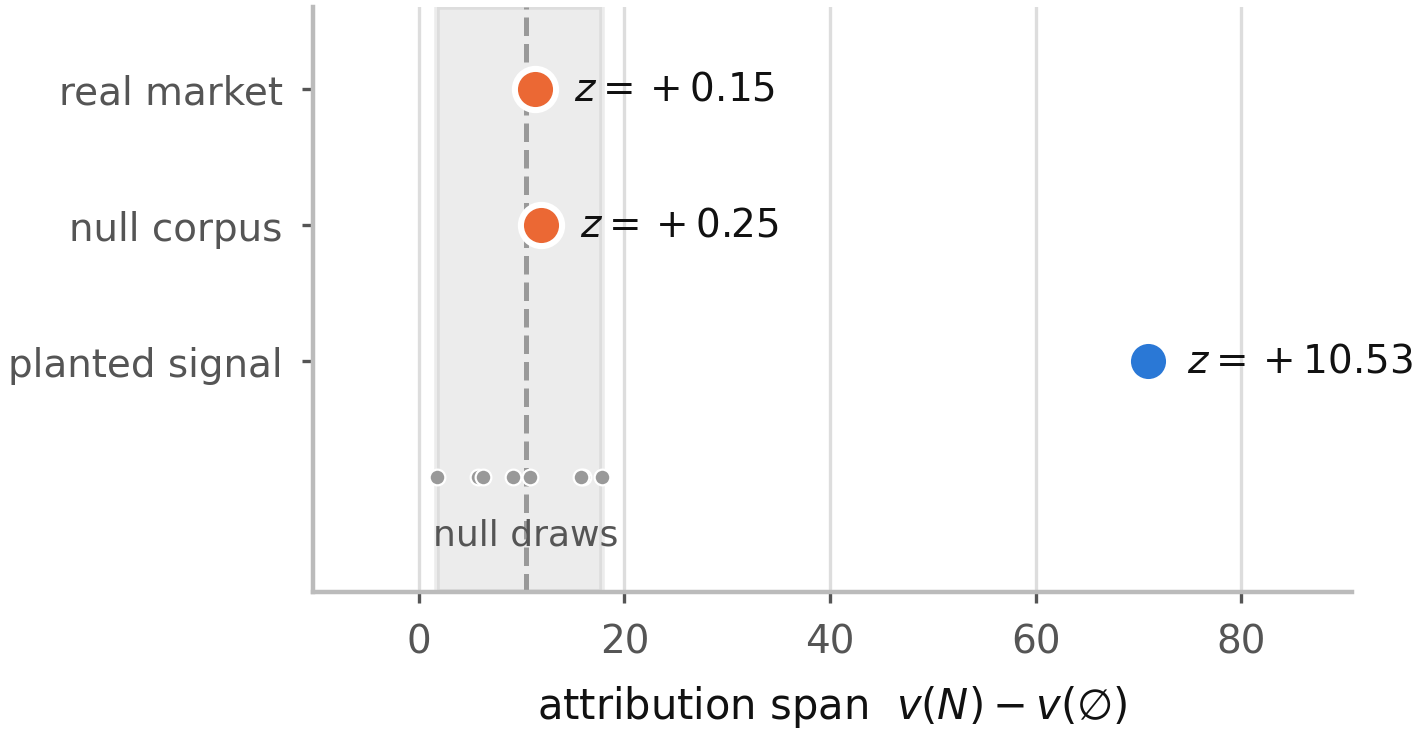
\includegraphics[width=\columnwidth]{figures/fig_null_test.png}
\caption{Attribution spans against the null. The band is the range over 24 agents
trained where the observation channel carries no information.}
\label{fig:null}
\end{figure}

We note one consequence for our own reporting. An earlier draft stated that ``the
whole observation is worth $+5.914$ per episode against being blind'' and
presented it as a finding. Blind agents produce $+8.19 \pm 5.11$. It was noise.

\subsection{A positive control on real data}

Every case above where the test fires is synthetic, which invites the objection
that it detects planted signal rather than information. Holding the corpus,
features, normalizer, split and null construction fixed and varying only the
objective answers it. The market's price is calibrated to $0.0172$, so it is
highly informative \emph{about the outcome} while offering nothing to trade
against once a $9\%$ round-trip fee is paid. Scoring the same architecture on
the same real episodes for \emph{calling} the settlement rather than trading it,
against a null of 24 agents trained on those episodes with observations
blinded, gives a span of $+7.46$ against $-0.48 \pm 2.34$: $z=+3.40$,
informative, unchanged in all $4{,}000$ resamples. The trading agent on
identical episodes and an identical null gives $+7.41$ against $+2.47 \pm 2.29$,
$z=+2.16$, which the two-part rule declines, though only $64\%$ of resamples
agree and we report it as borderline. The two spans are nearly the same size;
what separates them is the null, since a blind agent cannot call the outcome at
all but can still decline to trade. The market data is not uninformative. The
information is not monetisable, and an attribution of the trading agent cannot
tell those two situations apart.

\subsection{Validation against ground truth}

On the planted corpus, outcome attribution ranks the planted feature first with
$55\%$ of total mass. On the decoy corpus, an agent trained where the decoy
predicts the outcome (in-sample $+47.24$, held out $-6.83$) is explained on
episodes where the decoy is provably worthless: per-decision attribution gives
it $6.5\%$ of mass at rank 3 of 18, outcome-based attribution $1.1\%$ at rank
10. Both are true; the policy does key on the decoy. Per-decision attribution is
correct about behaviour and misleading about value.

\subsection{Parameter randomisation is an underpowered reference}

Randomising parameters is used two ways. \citet{adebayo2018sanity} degrade a
single explanation and ask whether it changes. Here we use it the other way, as
a source of reference draws against which a trained agent's span is placed,
which is the construction available to a practitioner wanting an RL null. The
two answer different questions, and in the full paper we run the canonical
version as well: it clears the explanation we show to be empty, on both
explanatory targets we tried, so passing it is not evidence that there is
anything to explain.

We build both nulls for the same task (Table~\ref{tab:nulls},
Figure~\ref{fig:nullcmp}). A randomly initialised policy behaves arbitrarily, so
masking its inputs moves return unpredictably and the reference distribution is
very wide. Across sixteen checkpoints the parameter null never exceeds $z=2.45$,
including on a converged CartPole policy scoring 404 of 500, while the
environment null reaches $z=+117.6$. The two disagree on five of the sixteen.

\begin{table}[t]
\centering\small
\caption{Null construction on four control tasks. MountainCar is degenerate under both: no policy in the budget reaches the goal.}
\label{tab:nulls}
\begin{tabular}{lrrr}
\toprule
Environment & Parameter & Environment & Ratio \\
\midrule
CartPole & $\pm \mathbf{138.92}$ & $\pm \mathbf{3.29}$ & $42\times$ \\
Acrobot & $\pm \mathbf{124.94}$ & $\pm \mathbf{0.00}$ & degenerate \\
MountainCar & $\pm \mathbf{0.00}$ & $\pm \mathbf{0.00}$ & $0\times$ \\
Pendulum & $\pm \mathbf{131.42}$ & $\pm \mathbf{37.79}$ & $3\times$ \\
\bottomrule
\end{tabular}
\end{table}

\paragraph{Why it is wide.} The gap has a mechanism, and it is not about
explanations. On every task the parameter null's width equals the spread of
random-initialisation return to three significant figures: $138.38$ against
$138.92$ on CartPole, $123.04$ against $124.94$ on Acrobot. In
$\Delta = \vfn(N) - \vfn(\emptyset)$ the masked term is near-constant for a
random network (sd $1.8\%$ of the unmasked term's on CartPole), because a policy
not using its observations loses little when they go. The span inherits the
unmasked variance entire: \emph{parameter randomisation measures the variance of
initialisation}, which is why a test built on it has no power.

\begin{figure*}[t]
\centering
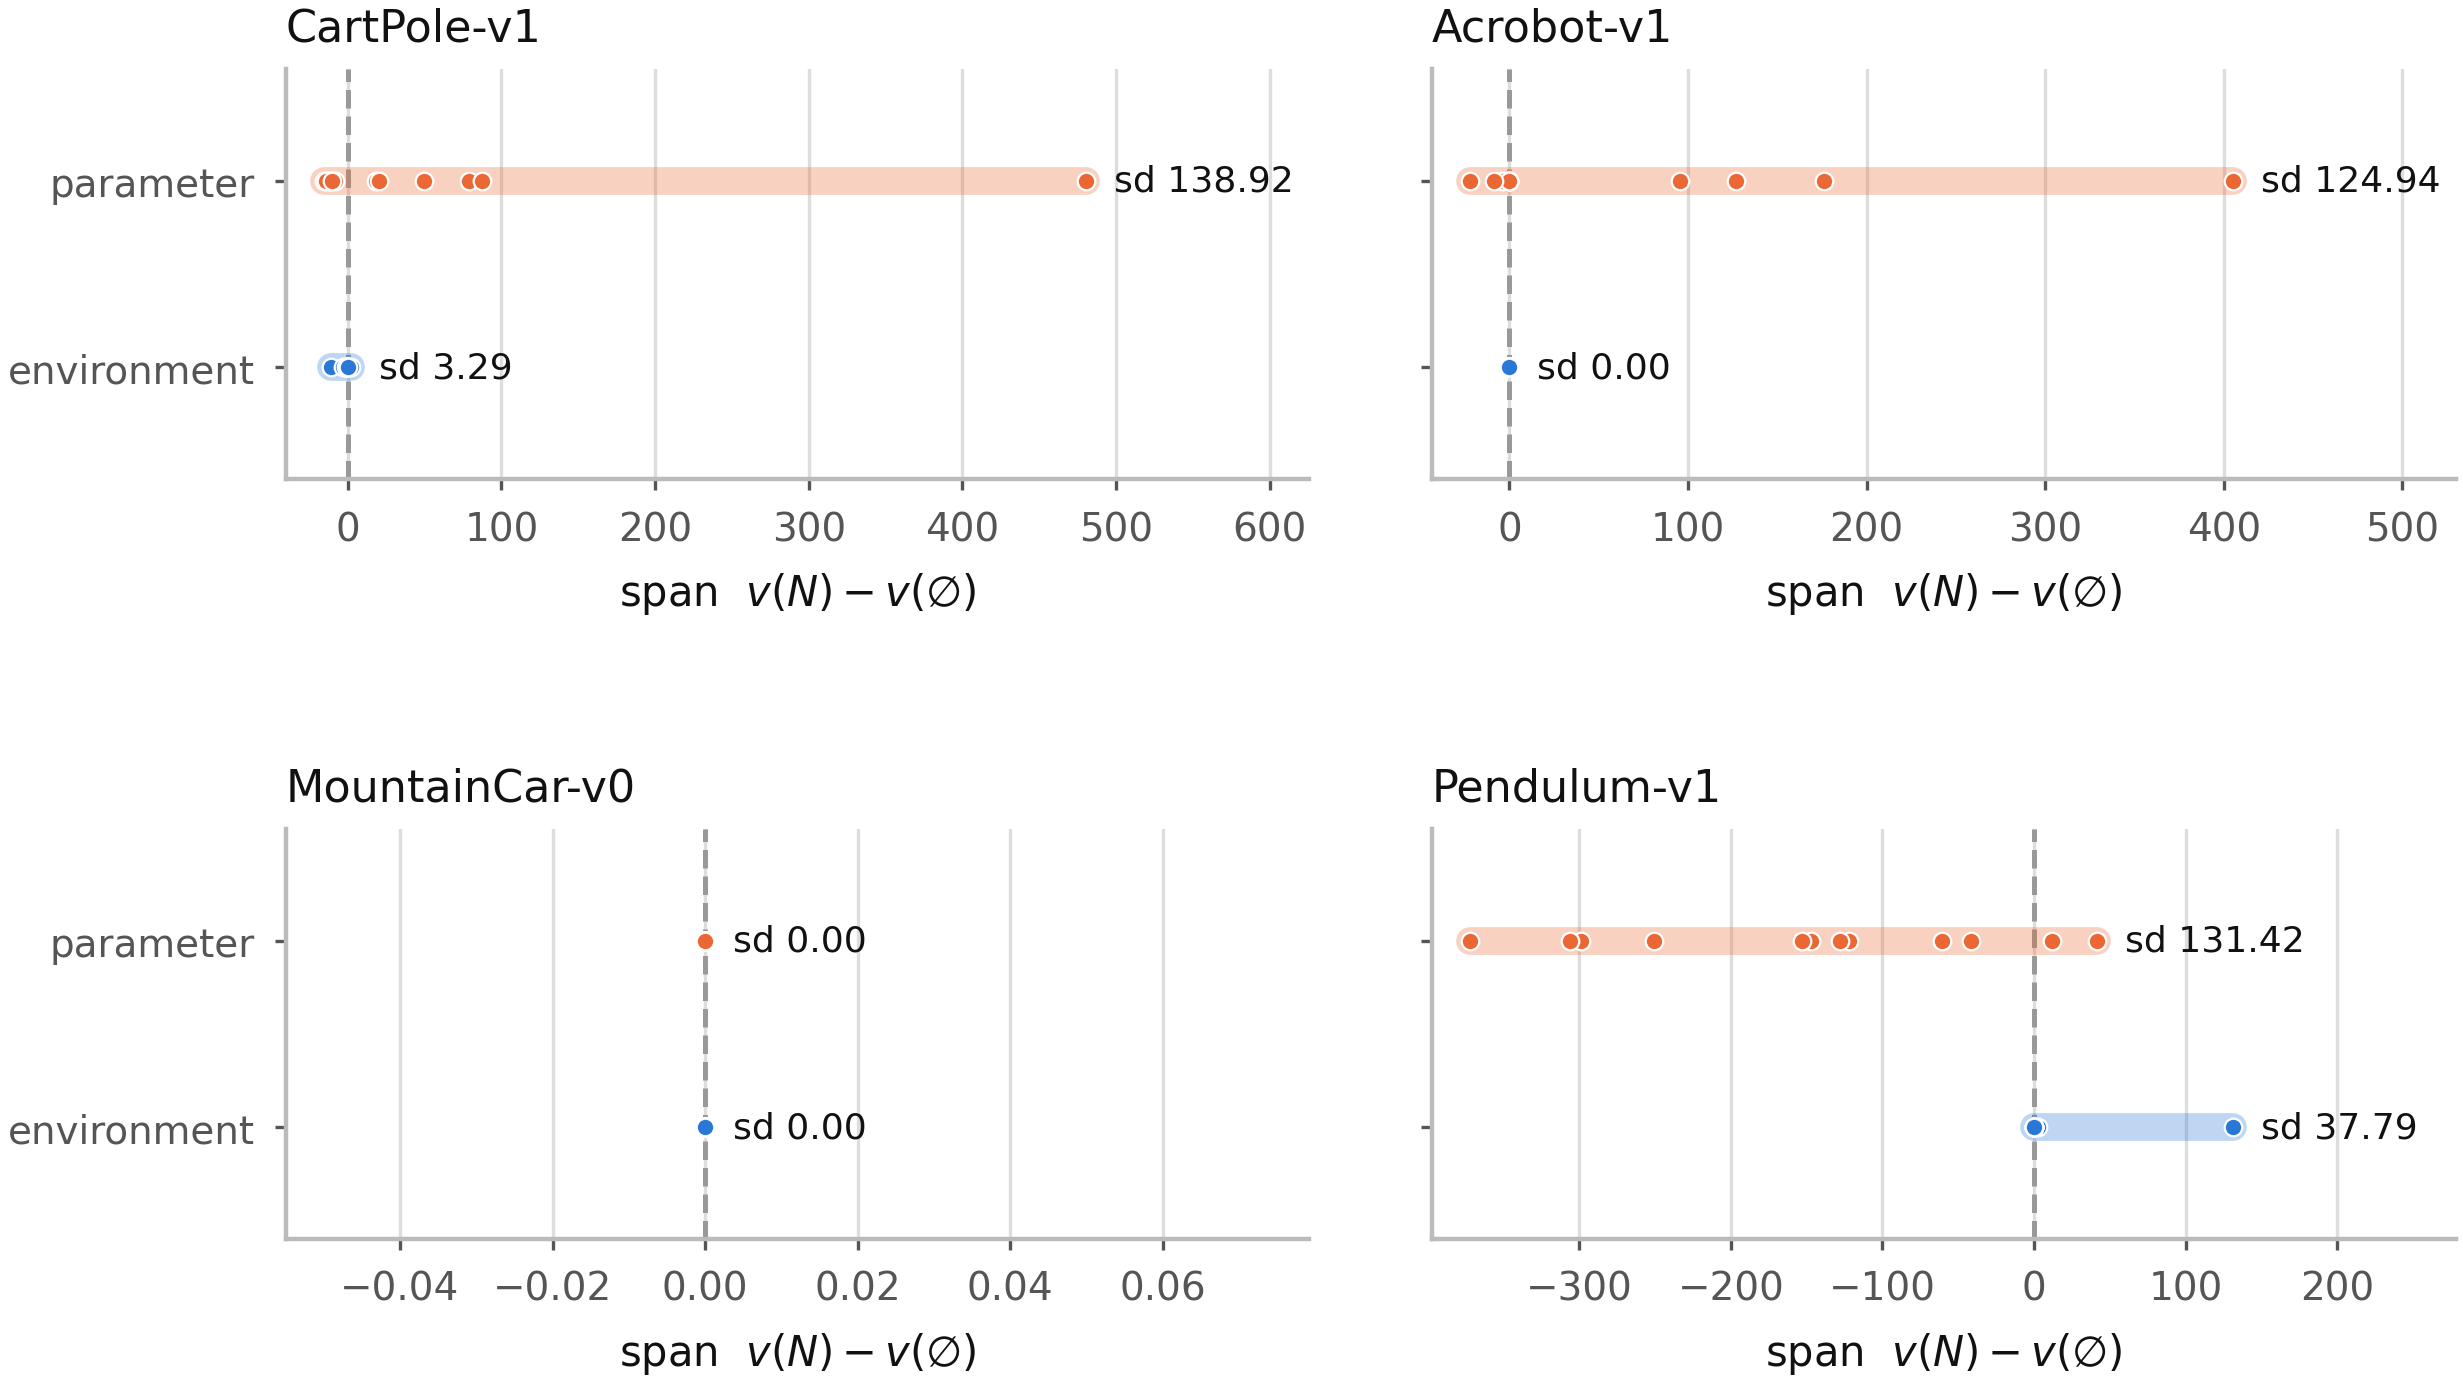
\includegraphics[width=\textwidth]{figures/fig_null_comparison.png}
\caption{Spread of each null construction. Width determines power: a very wide
reference distribution cannot reject anything.}
\label{fig:nullcmp}
\end{figure*}

Acrobot also shows the test tracking \emph{whether there is anything to explain}
rather than agent quality: its agent fails completely until it learns, the span
is exactly $0.00$ there, and the test correctly declines. CartPole's observations
matter at every skill level and the test fires throughout. We do not claim
undertrained agents generally produce empty explanations.

\subsection{Attribution is not identified by task performance}

We add a training penalty on the divergence between $\pi(\cdot\mid s)$ and
$\pi(\cdot\mid s')$, where $s'$ has one feature resampled from the batch
marginal: the same perturbation the attribution measures
(Table~\ref{tab:steer}).

\begin{table}[t]
\centering\small
\caption{Steering one feature's attribution.}
\label{tab:steer}
\begin{tabular}{lrrr}
\toprule
Corpus & Attribution & Return & $p$ \\
\midrule
market & $39.9\% \to \mathbf{3.2\%}$ & $-3.49 \to -1.65$ & $\mathbf{0.66}$ \\
planted signal & $46.5\% \to \mathbf{1.5\%}$ & $+45.04 \to \mathbf{+7.92}$ & $<$0.001 \\
\bottomrule
\end{tabular}
\end{table}


The attribution is equally suppressible in both cases. What differs is the price:
suppressing the planted signal destroys $81\%$ of return; on the market it costs
nothing measurable. Explanations are steerable at no cost exactly where they are
not tracking anything, corroborating Section 4.1 by a route sharing no machinery
with the null test. The control matters: had steering succeeded on both, the
penalty would merely be defeating the attribution method.

This differs from \citet{slack2020fooling}, who construct classifiers that detect
the off-manifold points LIME and SHAP query. Here the agent is trained normally
and the resulting explanation is \emph{correct} about the resulting model; the
point is that behaviour does not pin it down.

\subsection{Three replacements, three failures}
\label{sec:cost}

Our null trains its agents on synthetic signal-free corpora, so the corpus
varies along with the information. Two constructions hold it fixed instead, and
both fail.

\textbf{Blinding the observation channel} is what the definition above literally
says. Run on every case it produces a false positive: on a corpus built to
contain no informative feature, span $+13.90$ against a null of
$0.00 \pm 0.00$, which fires. Its verdict on the real market also flips with the
null agents' training budget, from $z=+0.55$ at 20 updates to $z=+203.6$ at 160,
as those agents converge. Blinding gives agents that cannot see; they converge
to a constant policy, whose return does not depend on its inputs at all, so
every null span is exactly zero. The agent under test is sighted, so the right
reference is sighted agents with nothing to learn.

\textbf{Permuting the outcomes} keeps them sighted and is the direct analogue of
the supervised test. Observations are untouched to the bit and the outcome rate
is preserved exactly. It has power ($z=+10.48$ on the planted signal) and
specificity ($z=+1.75$ on the signal-free corpus) and still fails: on the real
market the agent's span lands \emph{fifteen standard deviations below} its own
null, because the null agents earn $+36.26$ an episode where it earns $-1.13$.
The price forecasts the outcome, so relabelling leaves the forecast attached to
a different contract and the market becomes grossly mispriced. Fading the
terminal price, a rule needing only the quote, earns $-0.002$ per contract in
the real corpus and $+0.486$ in the permuted one. The null agents learn that
arbitrage and it requires seeing the price. Wherever an observation forecasts
the label, permuting the label makes the forecast exploitably wrong.

\textbf{The pattern.} Removing the information also perturbs something else, and
the perturbation decides the verdict: the corpus, the agent's responsiveness, or
the difficulty of the task. We keep the signal-free-corpus null because its
fault is the mildest and runs in the conservative direction, which is a reason
to trust our negative results more than our positive ones.

\section{Limitations}

The test adapts \citet{adebayo2018sanity}; the outcomes framing is
\citet{beechey2023sverl}'s. The span measures information in aggregate, not
whether the decomposition among features is right. Temporal credit assignment and
off-policy attribution are named, not solved; these are
FastSVERL's~\citep{beechey2025fastsverl} territory. An earlier mechanism we
proposed for the $42\times$ gap (that randomising weights perturbs the
measurement's domain and compounds along the trajectory) was tested and
rejected: over horizons 4 to 28 both nulls grow at indistinguishable rates
($\alpha=0.94$ against $0.83$). A variance decomposition accounts for it
instead, and involves no compounding. Four environments is too few to fit
a law, so we report that correspondence rather than a coefficient. The aggregate verdict also survives a
$k$-nearest-neighbour conditional masker that substantially reduces off-manifold
states, though the per-feature ranking does not, disagreeing there on the most
important feature. Accordingly the test validates whether there is something
outcome-relevant to explain, not which feature attribution is correct. Scope is
one real domain and four classic-control tasks, all with small observation
spaces, so nothing here speaks to pixel-based agents.

\section{Conclusion}

An attribution can be stable, precisely estimated, plausible, and empty. The
checks practitioners commonly apply do not detect this, because none of them
asks whether there was anything outcome-relevant to explain. A null-model test asks it directly, using a
statistic the attribution framework already provides. Building one is the hard
part: every construction we tried removes the information and perturbs something
else, and the perturbation decides the verdict.

\bibliographystyle{plainnat}
\bibliography{references}

\end{document}
